\tikzset{every picture/.style={line width=0.75pt}} %set default line width to 0.75pt        

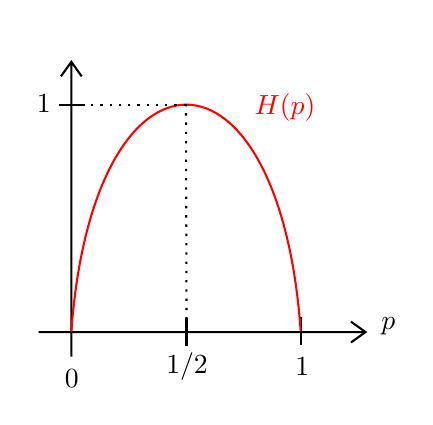
\begin{tikzpicture}[x=0.75pt,y=0.75pt,yscale=-1,xscale=1]
%uncomment if require: \path (0,300); %set diagram left start at 0, and has height of 300

%Shape: Axis 2D [id:dp03836096767914454] 
\draw  (184,209.7) -- (341.5,209.7)(199.75,79.5) -- (199.75,221.5) (334.5,204.7) -- (341.5,209.7) -- (334.5,214.7) (194.75,86.5) -- (199.75,79.5) -- (204.75,86.5)  ;
%Straight Lines [id:da09029121839767407] 
\draw    (310.25,202.5) -- (310.25,216) ;


%Straight Lines [id:da6499966939007862] 
\draw    (206.25,100.4) -- (193.75,100.4) ;


%Curve Lines [id:da6597373551550418] 
\draw [color={rgb, 255:red, 255; green, 0; blue, 0 }  ,draw opacity=1 ]   (199.75,209.5) .. controls (210.4,63.55) and (300,63.88) .. (310.25,209.25) ;


%Straight Lines [id:da4829975793327501] 
\draw    (255.25,203) -- (255.25,216.5) ;


%Straight Lines [id:da4265093472437165] 
\draw  [dash pattern={on 0.84pt off 2.51pt}]  (255,99.8) -- (255.25,204.5) ;


%Straight Lines [id:da9213182147125973] 
\draw  [dash pattern={on 0.84pt off 2.51pt}]  (255,100.2) -- (206.6,100.2) ;



% Text Node
\draw (352.5,207) node   {$p$};
% Text Node
\draw (302.7,101.6) node [color={rgb, 255:red, 255; green, 0; blue, 0 }  ,opacity=1 ]  {$H( p)$};
% Text Node
\draw (200,232) node   {$0$};
% Text Node
\draw (311,226.5) node   {$1$};
% Text Node
\draw (186.5,99.5) node   {$1$};
% Text Node
\draw (255.5,226.5) node   {$1/2$};


\end{tikzpicture}